\subsection{premi/client/editor}
\begin{figure}[h]
\begin{center}
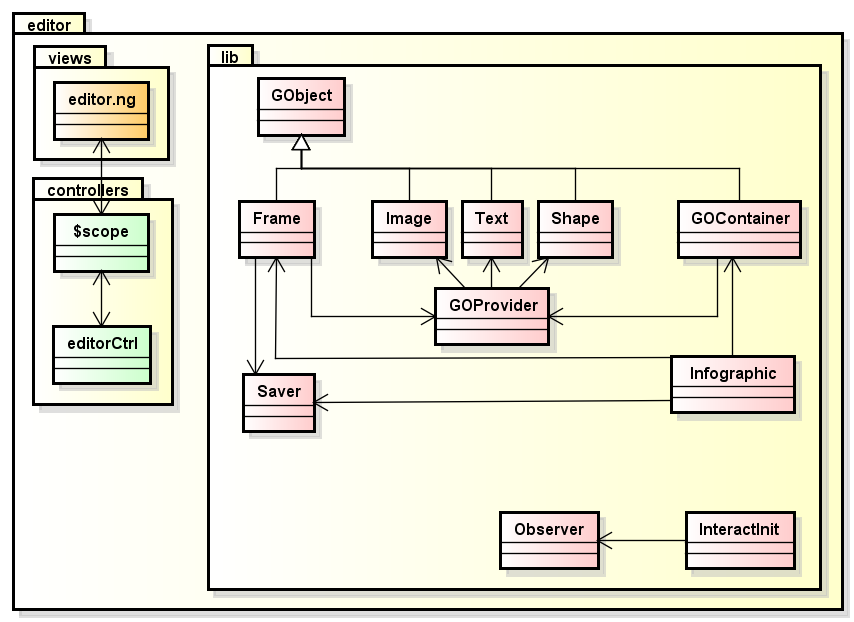
\includegraphics[scale=0.40]{img/diapkg/editor.png}
\caption{Diagramma della classe premi/client/editor}
\end{center}
\end{figure}

\subsubsection{premi/client/editor/lib/GObject}
\begin{figure}[h]
\begin{center}
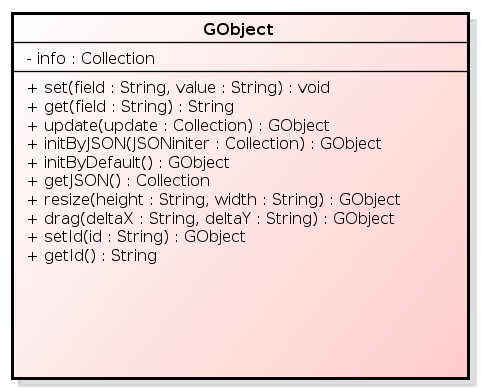
\includegraphics[scale=0.40]{img/diacla/GObject.png}
\caption{Diagramma della classe premi/client/editor/GObject}
\end{center}
\end{figure}

\begin{description}
%-------  descrizione della classe%
\item[Descrizione] \hfill \\
	GObject è una classe astratta che rappresenta un oggetto generico della presentazione. Contiene i metodi generali che caratterizzano ciascun oggetto grafico che può essere inserito in una presentazione.
	
%-------  lista degli Attributi%	
\item[Attributi] \hfill \\
	\begin{description}
		\item[\texttt{- info : Collection			}] \hfill \\
			info è un oggetto JSON che contiene i seguenti campi:
				\begin{itemize}
					\item \textit{\_id:} rappresenta l'id che identifica l'oggetto;
					\item \textit{dataX:} identifica la posizione orizzontale dell'asse x dell'oggetto;
					\item \textit{dataY:} identifica la posizione verticale dell'asse y dell'oggetto;
					\item \textit{dataZ:} identifica il grado di trasparenza dell'oggetto; %da chiedere%
					\item \textit{height:} identifica l'altezza dell'oggetto;
					\item \textit{width:} identifica la larghezza dell'oggetto;
					\item \textit{scale:} identifica la scala dell'oggetto; %da chiedere%
					\item \textit{lvl:} identifica il livello dell'oggetto. %da chiedere%
				\end{itemize}
					 
		
	\end{description}
	
	
%-------  lista dei metodi
\item[Metodi] \hfill \\

	% -- inizio metodo -- %
	\begin{description}
		\item[\texttt{+ set(field : String, value : String) : void			}] \hfill \\
			permette di settare un campo dell'attributo info.
			
		\begin{description}
			% -- lista argomenti del metodo -- %
			\item[Argomenti] \hfill \\
				\begin{itemize}
				
					\item \texttt{field : String			} \hfill \\
					field identifica il campo da settare di info;
					\item \texttt{value : String			} \hfill \\
					value rappresenta il valore del campo da settare su l'attributo info.
				\end{itemize}
		\end{description}

\end{description}

\begin{description}
		\item[\texttt{+ get(field : String) : String			}] \hfill \\
			restituisce il valore di un campo dell'attributo info.
			
		\begin{description}
			% -- lista argomenti del metodo -- %
			\item[Argomenti] \hfill \\
				\begin{itemize}
				
					\item \texttt{field : String			} \hfill \\
					field identifica l'attributo info di cui si vuole venga restituito il valore.
				\end{itemize}
		\end{description}

\end{description}

\begin{description}
		\item[\texttt{+ update(update : Collection) : GObject			}] \hfill \\
			permette di aggiornare i campi dell'attributo info.
			
		\begin{description}
			% -- lista argomenti del metodo -- %
			\item[Argomenti] \hfill \\
				\begin{itemize}
				
					\item \texttt{update : Collection			} \hfill \\
					update è un oggetto JSON che contiene chiave e valore dei campi che devono essere aggiornati. 
				\end{itemize}
		\end{description}

\end{description}

\begin{description}
		\item[\texttt{+ initByJSON(JSONiniter : Collection) : GObject			}] \hfill \\
			permette di inizializzare l'attributo info tramite un oggetto JSON. 
			
		\begin{description}
			% -- lista argomenti del metodo -- %
			\item[Argomenti] \hfill \\
				\begin{itemize}
				
					\item \texttt{JSONiniter : Collection			} \hfill \\
					è un oggetto JSON che contiene chiave e valore di inizializzazione dei campi dell'attributo info. 
				\end{itemize}
		\end{description}

\end{description}

\begin{description}
		\item[\texttt{+ initByDefault() : GObject			}] \hfill \\
			permette di inizializzare i campi dell'attributo info con i parametri di default. 

\end{description}

\begin{description}
		\item[\texttt{+ getJSON() : String			}] \hfill \\
			restituisce la collection dell'attributo info.

\end{description}

\begin{description}
		\item[\texttt{+ resize(height : String, width : String) : GObject			}] \hfill \\
			permette di settare l'altezza e la larghezza del'oggetto.
			
		\begin{description}
			% -- lista argomenti del metodo -- %
			\item[Argomenti] \hfill \\
				\begin{itemize}
				
					\item \texttt{height : String			} \hfill \\
					identifica il valore dell'altezza da settare sul campo height dell'attributo info;
					\item \texttt{width : String			} \hfill \\
					identifica il valore dell'altezza da settare sul campo width dell'attributo info;				
				\end{itemize}
		\end{description}
		
\end{description}

\begin{description}
		\item[\texttt{+ drag(deltaX : String, deltaY : String) : GObject			}] \hfill \\
			permette di settare la posizione dell'oggetto sull'asse x e y.
			
		\begin{description}
			% -- lista argomenti del metodo -- %
			\item[Argomenti] \hfill \\
				\begin{itemize}
				
					\item \texttt{deltaX : String			} \hfill \\
					identifica il valore della posizione sull'asse x da settare sul campo deltaX dell'attributo info.
					\item \texttt{deltaY : String			} \hfill \\
					identifica il valore della posizione sull'asse y da settare sul campo deltaY dell'attributo info;				
				\end{itemize}
		\end{description}
		
\end{description}

\begin{description}
		\item[\texttt{+ setId(id : String) : GObject			}] \hfill \\
			permette di modificare o di settare l'id dell'oggetto
			
		\begin{description}
			% -- lista argomenti del metodo -- %
			\item[Argomenti] \hfill \\
				\begin{itemize}
				
					\item \texttt{id : String			} \hfill \\
					identifica il valore dell'id da settare sul campo \_id dell'attributo info.
				\end{itemize}
		\end{description}
		
\end{description}

\begin{description}
		\item[\texttt{+ getId()			}] \hfill \\
			restituisce l'id dell'oggetto.
\end{description}


\end{description}

\subsubsection{premi/client/editor/lib/GOProvider}
\begin{figure}[h]
\begin{center}
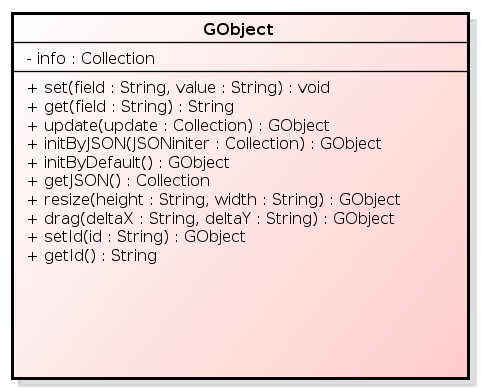
\includegraphics[scale=0.40]{img/diacla/GObject.png}
\caption{Diagramma della classe premi/client/editor/GObject}
\end{center}
\end{figure}

\begin{description}
%-------  descrizione della classe%
\item[Descrizione] \hfill \\
	GOProvider è una classe statica contiene i metodi per inizializzare gli oggetti image, text, shape che possono essere inseriti in un frame.
	
%-------  lista dei metodi
\item[Metodi] \hfill \\

	% -- inizio metodo -- %
	\begin{description}
		\item[\texttt{+ init(type : String) : GObject			}] \hfill \\
			inizializza con i parametri di default un oggetto image, shape o text e ne restituisce il riferimento.
			
		\begin{description}
			% -- lista argomenti del metodo -- %
			\item[Argomenti] \hfill \\
				\begin{itemize}
				
					\item \texttt{type : String			} \hfill \\
					identifica il tipo di oggetto da inizializzare.
				\end{itemize}
		\end{description}

\end{description}

	% -- inizio metodo -- %
	\begin{description}
		\item[\texttt{+ initByJSON(GO : Collection) : GObject			}] \hfill \\
			inizializza con un oggetto JSON, un oggetto image, text o shape e ne restituisce il riferimento.
			
		\begin{description}
			% -- lista argomenti del metodo -- %
			\item[Argomenti] \hfill \\
				\begin{itemize}
				
					\item \texttt{GO : Collection			} \hfill \\
					è un oggetto JSON che serve per inizializzare l'oggetto da resituire come riferimento.
				\end{itemize}
		\end{description}

\end{description}

\end{description}

\subsubsection{premi/client/editor/lib/frame}
\begin{figure}[h]
\begin{center}
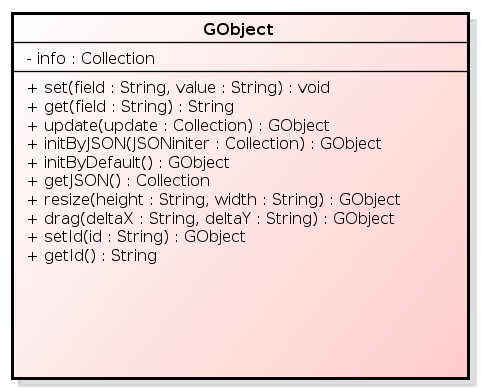
\includegraphics[scale=0.40]{img/diacla/GObject.png}
\caption{Diagramma della classe premi/client/editor/GObject}
\end{center}
\end{figure}

\begin{description}
%-------  descrizione della classe%
\item[Descrizione] \hfill \\
	frame è una classe che rappresenta un frame di una presentazione. E' un oggetto che può essere rappresentato nella presentazione. 
	
%-------  lista delle classi ereditate%	
\item[Classi ereditate] \hfill \\
	\begin{itemize}
		\item GObject
	\end{itemize}
	
%-------  lista degli Attributi%	
\item[Attributi] \hfill \\
	\begin{description}
		\item[\texttt{- info : Collection			}] \hfill \\
			l'attributo info è un oggetto JSON che estende l'attributo info ereditato da GObject. I campi aggiuntivi sono:
	\begin{itemize}
		\item \textit{backgroundColor:} rappresenta il colore di Background del frame;
		\item \textit{content:} è un oggetto JSON che contiene gli oggetti che fanno parte del frame;
		\item \textit{type:} identifica che l'oggetto trattato è un frame.
	\end{itemize}
	\end{description}
	\begin{description}
		\item[\texttt{- selectedGO : GObject			}] \hfill \\
			contiene l'oggetto GObject contenuto nel frame corrente selezionato dall'utente.  
	\end{description}
	\begin{description}
		\item[\texttt{- saver : Saver			}] \hfill \\
			contiene un oggetto saver che permette di interfacciarsi con il database.  
	\end{description}
	
%-------  lista dei metodi
\item[Metodi] \hfill \\

	% -- inizio metodo -- %
	\begin{description}
		\item[\texttt{- findNewId() : String			}] \hfill \\
			trova un nuovo id valido per il frame corrente.

\end{description}

	% -- inizio metodo -- %
	\begin{description}
		\item[\texttt{+ initByJSON(GO : Collection) : GObject			}] \hfill \\
			inizializza con un oggetto JSON, un oggetto image, text o shape e ne restituisce il riferimento.
			
		\begin{description}
			% -- lista argomenti del metodo -- %
			\item[Argomenti] \hfill \\
				\begin{itemize}
				
					\item \texttt{GO : Collection			} \hfill \\
					è un oggetto JSON che serve per inizializzare l'oggetto da resituire come riferimento.
				\end{itemize}
		\end{description}

\end{description}

\end{description}




